\section{Примеры из физики}
Обозначения: $\frac{\partial^2 u}{\partial t^2} = u_{tt}, \Delta = \partial_x^2 + \partial_y^2 + \partial_z^2$
\begin{enumerate}
	\item{Волновые уравнения.
			\[
				u_{tt} = a^2 u_{xx}
		\] - уравнение малых колебаний струны
		\[
				u_{tt} = a^2 u_{xx} + g
		\] - уравнение малых колебаний струны с учетом силы тяжести, где $g$ - потенциал массовой силы.
		\[
			u_{tt} = a^2 \left( u_{xx} + u_{yy}\right) + g
		\] - уравнение мембраны
		\[
			u_{tt} = a^2 \left( u_{xx} + u_{yy} + u_{zz}\right) + g
		\] - уравнение акустики
	}
\item{\[
			u_t = a^2 u_{xx} + g
	\] - уравнение теплопроводности для стержня.
	\[
		u_t = a^2 \left( u_{xx} + u_{yy}\right) + g
	\] - уравнение теплопроводности для пластины.
	\[
		u_t = a^2 \left( u_{xx} + u_{yy} + u_{zz}\right) + g
	\] - уравнение теплопроводности для тела.
}
\item{
		Уравнение Лапласа:
		\[
			\Delta u = 0
		\]
		Уравнение Пуассона:
		\[
			\Delta u = -g
		\]
	}
\item{
		Уравнение вибраций для стержня:
		\[
			u_{tt} + a^2 u_{xxxx} = g
		\]
		Для пластины:
		\[
			u_{tt} + a^2 \left(u_{xxxx} + 2 u_{xxyy} + u_{yyyy}\right) = g
		\]
	}
\item{
		Уравнение Шрёдингера (квантовая механика):
		\[
			i \hslash u_t = Hu
		\]
		где $i$ - мнимая единица, $\hslash$ - постоянная Планка, $H$ - оператор Гамильтона. Для одномерной частицы получится:
		\[
			H = E_\text{К} + E_\text{П}
		\]
		В классической механике это будет:
\[
	E_\text{К} = \frac{mv^2}{2} = \frac{m\left| \left| \overline{v}\right| \right|^2}{2} = \frac{\left| \left| \overline{P}\right| \right|^2}{2m}
\]
В квантовой механике:
\[
	\begin{aligned}
		\overline{P} = -i \hslash \nabla \\
		E_\text{К} = -\frac{\hslash^2}{2m} \Delta
	\end{aligned}
\]
То есть $E_\text{К}$ - это оператор. $E_\text{П}$ - потенциал внешнего поля, $E_\text{П}u = U(x) \cdot u$. Получили уравнение:
\[
	i \hslash u_t = -\frac{\hslash^2}{2m} u_{xx} + U(x) \cdot u
\] - нерелятивистская одномерная частица.
	}
	\begin{comment}
	\item{
			Уравнение ОТО (общая теория относительности)
			\[
				\begin{aligned}
					g_{vm} = \begin{pmatrix} c^2 & 0 & 0 & 0 \\ 0 & -1 & 0 & 0 \\ 0 & 0 & -1 & 0 \\ 0 & 0 & 0 & -1\end{pmatrix}	
				\end{aligned}
			\]
			Вот это метрический тензор.
		}
	\end{comment}
	\item{
			Уравнение Навье--Стокса. Уравнение для вязкой несжимаемой жидкости:
			\[
				\begin{aligned}
				\overline{w}_t = \underbrace{-\left( \overline{w}, \nabla\right) \overline{w}}_{\text{перенос жидкости}} + \underbrace{a^2 \Delta \overline{w}}_\text{вязкость} - \frac{1}{\underbrace{\rho}_{\text{плотность}}} \nabla \underbrace{P}_{\text{давление}} + \underbrace{g}_{\text{потенциальная массовая сила}} \\
				\mathrm{div} ~ \overline{w} = 0
			\end{aligned}
			\]
			при этом
			\[
				\begin{aligned}
					P = P(t,x,y,z) \in \mathbb{R}^1 \\
					\overline{w} = \overline{w} (t,x,y,z) \in \mathbb{R}^3
				\end{aligned}
			\]
		}
\end{enumerate}
\section{Одномерная частица в потенциальной яме}
Рассмотрим уравнение квантовой механики:
\[
	\begin{aligned}
	i \hslash u_t = Hu \\
	i \hslash u_t = -\frac{\hslash^2}{2m} u_{xx} + U(x) \cdot u
\end{aligned}
\]
где $U$ - потенциал:

\begin{figure}[H]
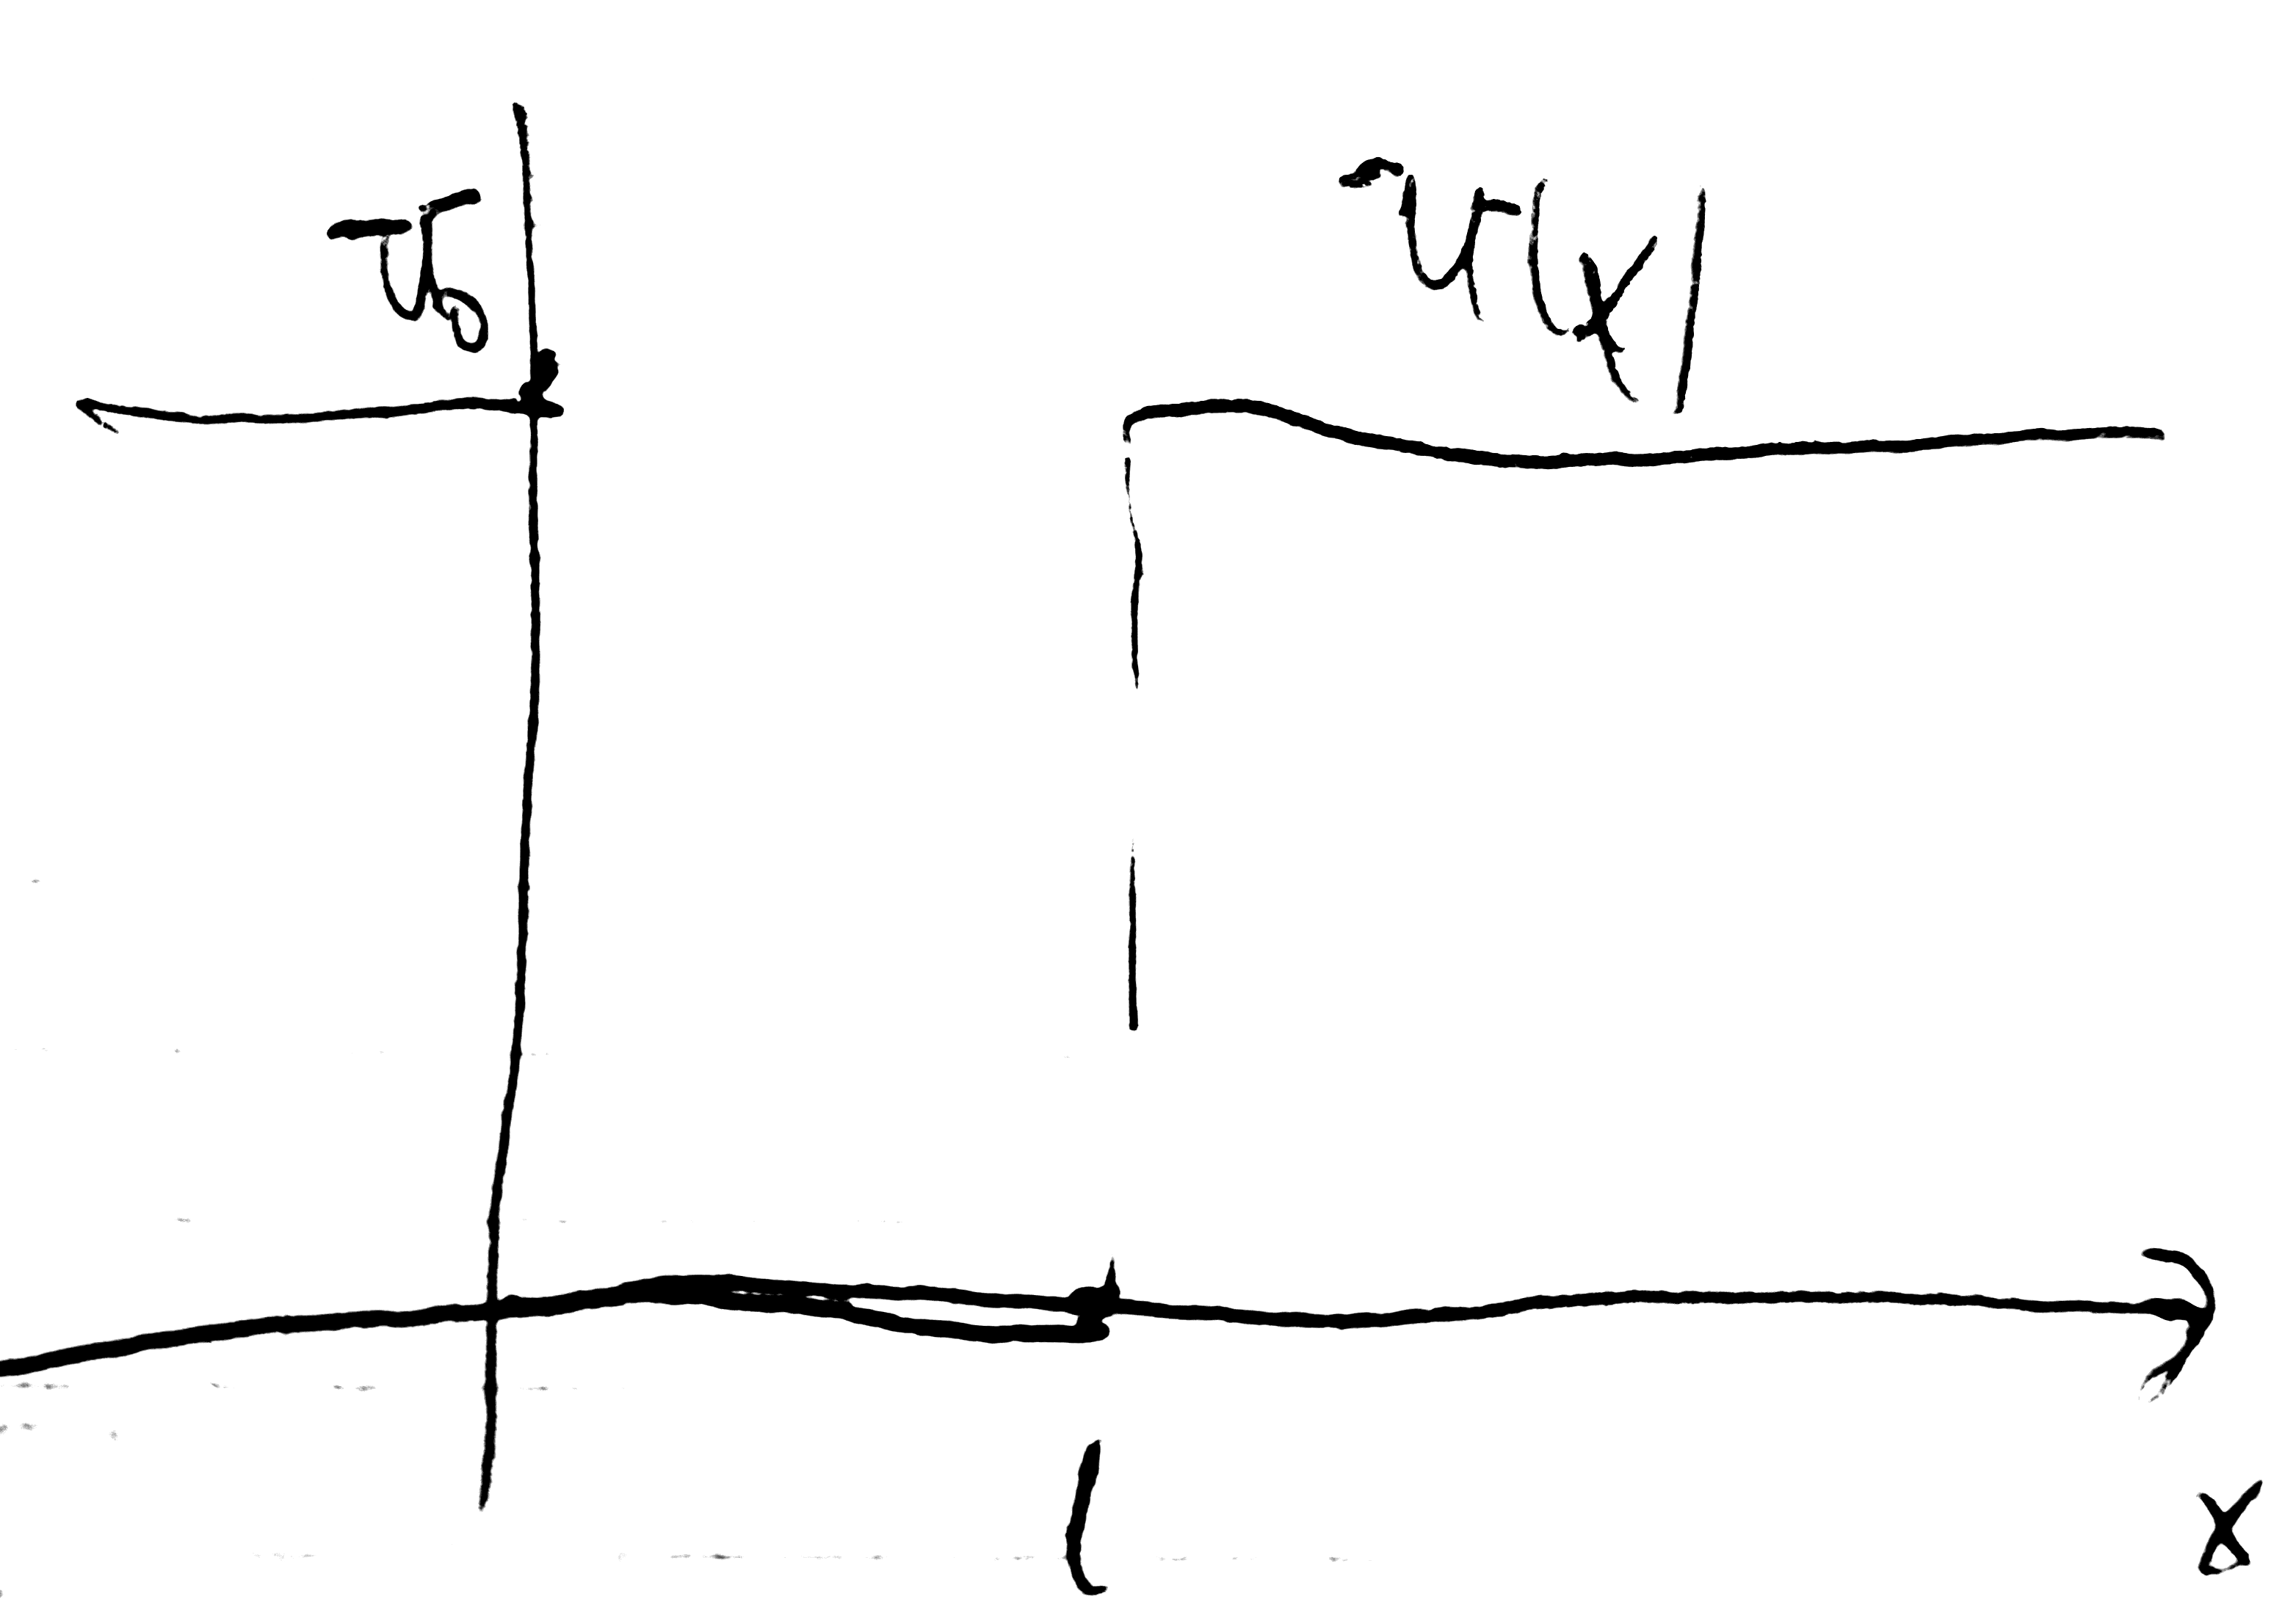
\includegraphics[width=\textwidth]{3}
\end{figure}

Дополнительные условия:

$u$ - гладкая функция,
\[
\int\limits_{-\infty}^\infty \underbrace{\left| u(x, t)\right|^2}_{\substack{\text{амплитуда вероятности} \\ \text{плотность распределения обнаружения частицы в }x}} \mathrm{d}x = 1
\]
Ищем решения диффура в виде:
\[
	\begin{aligned}
	u(x,t) = e^{i\left( \omega t + \varphi\right)} F(x) \\
	\omega = -\frac{E}{\hslash} \\
	E := -\omega \hslash \\
	u(x,t) = e ^{-i\frac{E}{\hslash} t + i \varphi} F(x) \\
	EF(x) = -\frac{\hslash^2}{2m} F''(x) + U(x) F(x)
	\end{aligned}
\]
где $F(x)$ - вещественная. (потому что как в ряде Фурье, из комбинаций вещественных функций можно собрать любую комплексную, но это не строгие суждения - строгие бы заняли не одну лекцию...)

Пусть $\frac{\hslash^2}{2m} = 1$ для простоты (мы всегда можем сделать такую систему координат, в которой это правда). Тогда:
\[
	F''(x) = \left\{ \begin{aligned}
			\overbrace{\left(U_0 - E\right)}^{>0} F(x), ~& x < 0 \\
			\overbrace{-E}^{<0}F(x), ~& x \in (0, l) \\
			\underbrace{\left(U_0 - E\right)}_{>0}F(x), ~& x > l
	\end{aligned}\right.
\]
Решаем обыкновенный диффур. Пусть $E \in (0, U_0)$.
\[
	F(x) = \left\{ \begin{aligned}
			c_1 e^{\sqrt{U_0-E} x} + c_2 e^{-\sqrt{U_0-E}x}, ~& x < 0 \\
			c_3 \cos \left( \sqrt{E}x\right) + c_4 \sin \left( \sqrt{E} x\right), ~& x \in (0, l) \\
			c_5 e^{\sqrt{U_0-E}x} + c_6 e^{-\sqrt{U_0-E}x}, ~& x > l
	\end{aligned}\right.
\]
Из <<дополнительных условий>>:
\[
	\begin{aligned}
		F - \text{гладкая} \\
		\int\limits_{-\infty}^{\infty} \left| u(x,t)\right|^2 \mathrm{d}x = \int\limits_{-\infty}^{\infty} F^2(x)\mathrm{d}x = 1
	\end{aligned}
\]
Самый последний интеграл сходится, поэтому можно сказать, что на бесконечности $F(x)$ должна быть нулевой $\implies c_2=c_5=0$.

Ещё должно быть 4 условия непрерывности:
\[
	\begin{aligned}
	F(+0)=F(-0) \\
	F'(+0)=F'(-0) \\
	F(l+0)=F(l-0) \\
	F'(l+0)=F'(l-0)
\end{aligned}
\]
Подставим в уравнения:
\[
	\left\{
	\begin{aligned}
		c_1 = c_3 \\
		c_1 \sqrt{U_0 - E} = c_4 \sqrt{E} \\
		c_3 \cos \left( \sqrt{E} l\right) + c_4 \sin \left( \sqrt{E}l\right) = c_6 e^{-\sqrt{U_0-E}l} \\
		-c_3 \sqrt{E} \sin \left( \sqrt{E} l\right) + c_4 \sqrt{E} \cos \left(\sqrt{E} l \right) = -c_6 \sqrt{U_0 - E} e^{-\sqrt{U_0 - E}l}
	\end{aligned}
	\right.
\]
Пусть 
\[
	\varepsilon = \sqrt{\frac{U_0-E}{E}}
\]
Тогда
\[
	\left\{
	\begin{aligned}
		c_1 = c_3 \\
		c_1 \varepsilon = c_4  \\
		c_1 \cos \left( \sqrt{E} l\right) + c_1 \varepsilon \sin \left( \sqrt{E}l\right) = c_6 e^{-\sqrt{U_0-E}l} \\
		-c_1 \sin \left( \sqrt{E} l\right) + c_1 \varepsilon \cos \left(\sqrt{E} l \right) = -c_6 \varepsilon e^{-\sqrt{U_0 - E}l}
	\end{aligned}
	\right.
\]
Рассмотрим последние два уравнения:
\[
	\left\{
		\begin{aligned}
		c_1 \cos \left( \sqrt{E} l\right) + c_1 \varepsilon \sin \left( \sqrt{E}l\right) = c_6 e^{-\sqrt{U_0-E}l} \\
		-c_1  \sin \left( \sqrt{E} l\right) + c_1 \varepsilon \cos \left(\sqrt{E} l \right) = -c_6 \varepsilon e^{-\sqrt{U_0 - E}l}
	\end{aligned}
	\right.
\]
В них неизвестные $c_1, c_6, E$. $c_1^2 + c_6^2 \ne 0$, т.к. иначе получим нулевое решение. В матричном виде будет:
\[
	\begin{pmatrix} \cos \left( \sqrt{E} l\right) + \varepsilon \sin \left( \sqrt{E} l\right) & -e^{-\sqrt{U_0-E}l} \\ \varepsilon \cos \left( \sqrt{E} l\right) - \sin \left( \sqrt{E} l\right) & \varepsilon e^{-\sqrt{U_0-E}l}\end{pmatrix} \begin{pmatrix} c_1 \\ c_6\end{pmatrix} = \begin{pmatrix} 0 \\ 0\end{pmatrix}
\]
Для существования решения необходимо, чтобы определитель матрицы слева был нулевой.

Ещё одна константа получится из условия на $\int=1$.

Получится небольшое число корней - уровни энергии для частицы. И частица может быть только на конкретном числе раздичных уровней. Вероятность частицы выпрыгнуть из потенциальной ямы тем больше, чем выше её уровень энергии. Но $\forall E > U_0$ квантование прекращается, и любые уровни энергии достижимы.
